\documentclass{beamer} \usepackage{graphicx,amsmath,amsfonts,amssymb,listings,tikz} \usepackage{multimedia}
\usetheme{Montpellier}
\usecolortheme{beaver}
\beamerdefaultoverlayspecification{<+->}

\begin{document}

\section{Article Review}
\title{Article Review - Multi-resolution dynamic mode decomposition for foreground/background
separation and object tracking \\ Week 9, Spring 2019}
\author{Brandon Gusto} %
\institute{Dept. of Scientific Computing \\ Florida State University}
\date{\today}
\frame{\titlepage}

\begin{frame}{Introduction}
    \centering
    Dynamic Mode Decomposition provides spatio-temporal modes that correlate
    data across spatial features (like PCA), but also pins the spatially
    correlated data to unique temporal Fourier modes.
\end{frame}

\begin{frame}{Overview}
    The task is to approximate nonlinear system
    \begin{figure}
        \center
        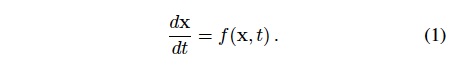
\includegraphics[scale=0.5]{linearsys.png}
    \end{figure}
    with
    \begin{figure}
        \center
        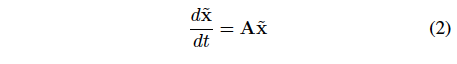
\includegraphics[scale=0.5]{approx.png}
    \end{figure}
    with the solution being
    \begin{figure}
        \center
        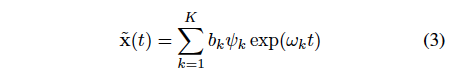
\includegraphics[scale=0.5]{solution.png}
    \end{figure}
    This is done in a least-square sense. The result is a low-rank structure,
    allowing for dimensionality reduction of the original system.
\end{frame}
    
\begin{frame}{Method}
    The DMD is a data-driven method, taking $M$ snapshots with $N$ spatial
    points saved per snapshot. These are stored in large data matrices
    \begin{figure}
        \center
        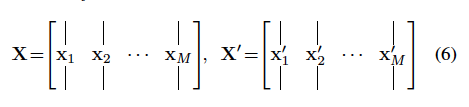
\includegraphics[scale=0.5]{data.png}
    \end{figure}
    where $X$ is the original data, and $X'$ is the data after some evolution of
    the nonlinear system. One can think of the DMD modes as the
    eigenvectors of $A = X' X^{\dagger}$. Here $A$ is the Koopman operator,
    central to the DMD, but too `mathy' for right now...
\end{frame}

\begin{frame}{Algorithm}
    First, an SVD of the original data set is computed
    \begin{figure}
        \center
        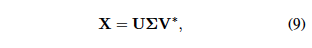
\includegraphics[scale=0.5]{svd.png}
    \end{figure}
    The SVD is truncated by retaining largest singular values and corresponding
    modes. An approximation $\widetilde{A}$ of the Koopman operator $A$ is given
    by projecting $A$ onto the low-rank modes of $U$:
    \begin{figure}
        \center
        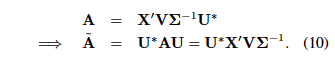
\includegraphics[scale=0.5]{koopman.png}
    \end{figure}
\end{frame}

\begin{frame}{Algorithm}
    Then an eigendecomposition of $\widetilde{A}$ is done
    \begin{figure}
        \center
        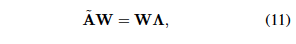
\includegraphics[scale=0.5]{eigen.png}
    \end{figure}
    and the ultimate goal is to reconstruct the eigendecomposition of $A$ from
    these eigenvectors and eigenvalues. Thus the eigenvectors of $A$ (DMD modes)
    are given by the columns of
    \begin{figure}
        \center
        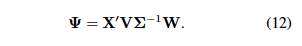
\includegraphics[scale=0.5]{dmdmodes.png}
    \end{figure}
    Using these modes as a basis, a projected evolution of the system in time is
    given by
    \begin{figure}
        \center
        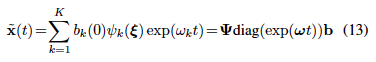
\includegraphics[scale=0.5]{predicted.png}
    \end{figure}
\end{frame}

\begin{frame}{Multiresolution}
    Multiresolution adds another flavor to DMD. Whereas in the standard method
    the spatially correlated data is represented in terms of Fourier modes, the
    multiresolution approach separates the DMD analysis into varying levels of
    time resolution. This has the benefit not allowing a single set of modes
    that dominate the SVD to marginalize features at other time scales.

\end{frame}

\begin{frame}{Multiresolution}
    \begin{figure}
        \center
        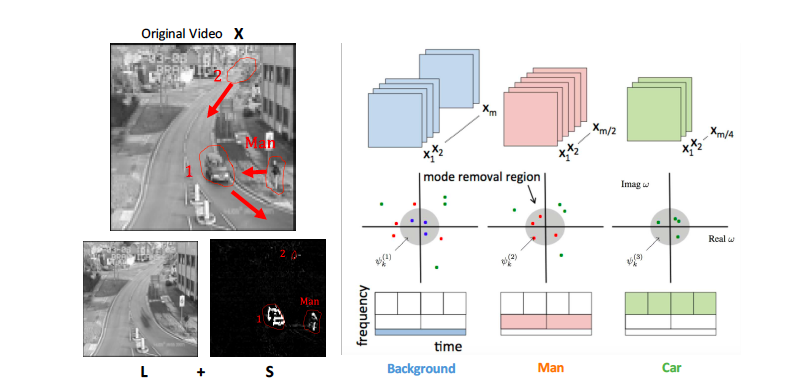
\includegraphics[scale=0.3]{example.png}
    \end{figure}
\end{frame}

\end{document}
